%% Overleaf			
%% Software Manual and Technical Document Template	
%% 									
%% This provides an example of a software manual created in Overleaf.

\documentclass{ol-softwaremanual}

% Packages used in this example
\usepackage{graphicx}  % for including images
\usepackage{microtype} % for typographical enhancements
\usepackage{minted}    % for code listings
\usepackage{amsmath}   % for equations and mathematics
\setminted{style=friendly,fontsize=\small}
\renewcommand{\listoflistingscaption}{List of Code Listings}
\usepackage{hyperref}  % for hyperlinks
\usepackage[a4paper,top=4.2cm,bottom=4.2cm,left=3.5cm,right=3.5cm]{geometry} % for setting page size and margins

% Custom macros used in this example document
\newcommand{\doclink}[2]{\href{#1}{#2}\footnote{\url{#1}}}
\newcommand{\cs}[1]{\texttt{\textbackslash #1}}

% Frontmatter data; appears on title page
\title{Hotel reservation system }
\version{1.0.0}
\author{Trinh Xuan Tam}
\softwarelogo{
\includegraphics[width=8cm]{logo}}

\begin{document}

\maketitle

\tableofcontents
% \listoflistings
\newpage

\section{Assignment}

Design domain model (diagram and technical document) for Hotel
reservation system which will support the following functions:

\begin{itemize}
  \item User will get a list of all different types of rooms.
  \item User selects a room type and check the room availability between the specified dates.
  \item User Makes Reservation.
\end{itemize}

\section{Business analysis}

\subsection{Domain definition}

The hotel reservation system is an platform designed to simplify the process of finding and booking hotel accommodations. It primarily assists guests in looking for a secure place to stay based on their preferences and time preferences. The core functionality of the system is centered around enabling users to view various types of available rooms, check the availability of these rooms for specific dates, and proceed with making reservations based on real-time data.

The system consists of several key entities that interact with each other. Users of the system, who can be guests or potential guests, initiate interactions by browsing room types that the hotel offers. Each room type, such as single, double, or suite, is distinctively defined by its features, capacity, and amenities, catering to different guest needs and expectations. The actual rooms, represented in the system as unique entities linked to their respective types, have specific characteristics such as room number, floor location, and maintenance status.

The reservation process begins when a user selects a room type and inputs their intended stay dates. The system then checks the availability of rooms matching the selected type during the specified period. If available, the user can proceed to make a reservation. This involves capturing detailed information such as the check-in and check-out dates, the number of occupants, and payment details. The system finalizes the booking by confirming the reservation and updating the room's availability status accordingly.

\pagebreak

\subsection{Analytical domain model}

\begin{figure}[h]
\centering
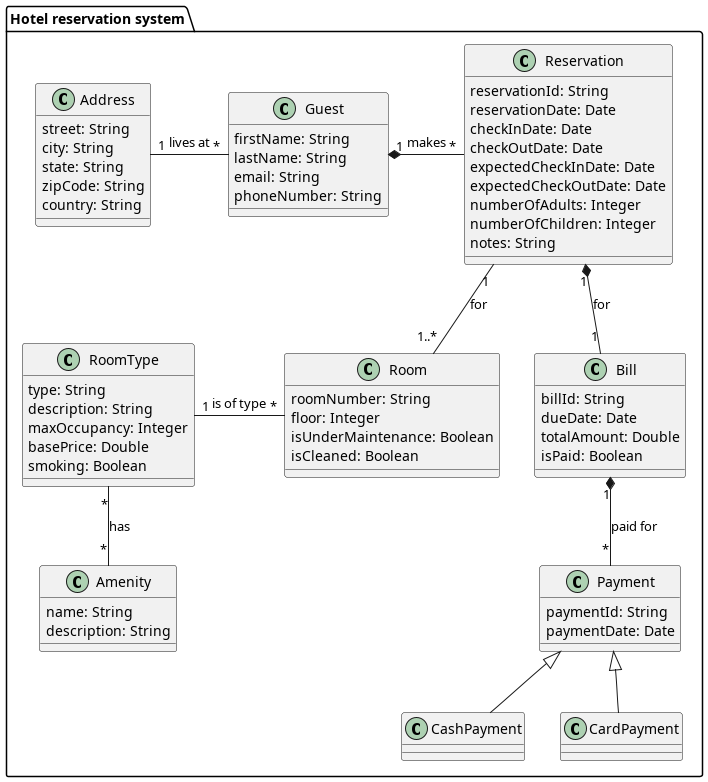
\includegraphics[width=0.9\textwidth]{images/domain-model.png}
\caption{\label{fig:domain-model} Domain model of the hotel reservation system.}
\end{figure}

The diagram illustrates a conceptual domain model, based to the specifications of the assignment. It is assumed that the system is being integrated with a singular hotel --- the model does not incorporate a distinct entity for the hotel. For the sake of simplicity and to stay within the scope of the assignment, operational entities such as maintenance schedules and employee management structures have been intentionally omitted.

\pagebreak

\subsubsection{Rooms}

Within the hotel reservation system domain model, the \texttt{Room} entity represents the various accommodation spaces available to guests. Each Room is assigned a \texttt{roomNumber}, serving as a unique identifier that facilitates the differentiation of rooms and supports the administrative aspects of bookings and maintenance. The floor attribute specifies the room's location by level, addressing preferences for particular views or access requirements. The primary factor determining room availability is the fact, whether it is currently reserved for a given time frame, with the reservation status taking precedence over other considerations. Moreover, the \texttt{isUnderMaintenance} attribute indicates if the room is out of service for repair or refurbishment, while the \texttt{isCleaned} attribute confirms that the room has been prepared according to the hotel's cleanliness protocols and is ready for new occupants.

The \texttt{RoomType} entity provides a classification system for rooms based on shared attributes and features. This classification aids users in finding rooms that match their preferences by offering a clear depiction of each room category. Essential characteristics such as type, \texttt{description}, \texttt{maxOccupancy}, \texttt{basePrice}, and \texttt{smoking} convey vital information about the rooms. While the \texttt{description} attribute offers insights into the room's amenities and layout, the \texttt{type} attribute describes the kind of room --- be it a single, double, or suite. The \texttt{maxOccupancy} attribute informs guests of the room's capacity, \texttt{basePrice} indicates the starting cost of the room, and the \texttt{smoking} attribute designates whether smoking is permitted, allowing guests to align their selection with their needs and desires.

The \texttt{Amenity} entity outlines the supplementary features and services that are linked to the \texttt{RoomTypes}, thereby enriching the guest experience. Amenity offerings, such as Wi-Fi, breakfast inclusion, or gym access, are described by their name and description and are consistent across all rooms within a particular \texttt{RoomType}. This design ensures uniformity in the amenities provided, simplifying the booking process and helping guests to make informed decisions based on the available room features.

\pagebreak

\subsubsection{Reservations}

The entity \texttt{Reservation} captures all the necessary information to book a guest's stay at the hotel. It holds a unique \texttt{reservationId} for each reservation, which serves as the primary key for retrieval and management. The entity also records the number of guests staying via \texttt{numberOfAdults} and \texttt{numberOfChildren}, ensuring the accommodation can meet the space requirements of the party.

Key dates are pivotal within the Reservation entity, with \texttt{checkInDate} and \texttt{checkOutDate} defining the actual stay period. Additionally, the attributes \texttt{expectedCheckInDate} and \texttt{expectedCheckOutDate} can be used for anticipated arrival and departure planning, which is particularly useful for managing hotel occupancy and resource allocation. The \texttt{notes} attribute provides space for any special requests or additional information pertinent to the guest's experience.

Tightly linked to the \texttt{Reservation} is the \texttt{Guest} entity, which details the personal information of the individual making the reservation. This includes \texttt{firstName}, \texttt{lastName}, \texttt{email}, \texttt{phoneNumber} and address information facilitating communication and personalized service.

\subsubsection{Payments}

Each reservation entity is accompanied by a corresponding bill, a vital component ensuring the integrity of every reservation. The completeness of the bill uses the following attributes: \texttt{dueDate}, \texttt{totalAmount}, and \texttt{isPaid}. The \texttt{dueDate} defines the latest date before the reservation will get cancelled by the system if the bill is not paid.

Additionally, a single bill may encompass multiple linked payments, facilitating a comprehensive tracking of payment history.

\end{document}
